% ==========================================================================
%  Computational grid sa_mi_baseline.su2: (a) whole grid,
%  (b) near-wall grid at the stagnation point.
%
%  Standalone LaTeX document: on Overleaf replace ALL of main.tex with this
%  file and compile with pdfLaTeX; include the compiled PDF in the paper.
%  Generated by make_mesh_figure.py from data/mesh_r_i.txt and
%  data/mesh_phi_j.txt (written and verified by check_mesh.py).
%  Grid: 294 x 520 cells, exact polar O-grid, symmetric about y = 0;
%  R = 38.1 mm, inlet r = 150.387 mm, dphi = 0.25 deg; radial spacing: first cell
%  0.122 um, ratio 1.15 to r = 39.440 mm, uniform 0.2005 mm to r = 75.534 mm,
%  ratio 1.05 to the inlet.
%  Lines shown: (a) every 4th line in each direction; (b) every grid line.
% ==========================================================================
\documentclass[border=1pt]{standalone}
\usepackage[T1]{fontenc}
\usepackage[scaled=0.92]{helvet}
\renewcommand{\familydefault}{\sfdefault}
\IfFileExists{newtxsf.sty}{\usepackage{newtxsf}}{}
\usepackage{tikz}
\usetikzlibrary{arrows.meta}
\definecolor{ink}{HTML}{000000}
\definecolor{bodygrey}{HTML}{D9D9D9}
\definecolor{accent}{HTML}{C0392B}
\definecolor{dimgrey}{HTML}{555555}
\tikzset{
  grid/.style={draw=ink, line width=0.22pt},
  wall/.style={draw=ink, line width=1.0pt},
  edge/.style={draw=ink, line width=0.6pt},
  frame/.style={draw=ink, line width=0.5pt},
  tick/.style={draw=ink, line width=0.45pt},
  ticklbl/.style={font=\sffamily\small, inner sep=1pt},
  axlbl/.style={font=\sffamily\small, inner sep=1pt},
  panel/.style={font=\sffamily\bfseries\small, inner sep=0pt},
  note/.style={font=\sffamily\footnotesize, inner sep=0.7pt, align=center, fill=white},
  zoom/.style={draw=accent, line width=0.8pt},
  dim/.style={draw=dimgrey, line width=0.45pt,
              {Stealth[length=1.5mm, width=1mm]}-{Stealth[length=1.5mm, width=1mm]}},
}

\begin{document}
\sffamily\small
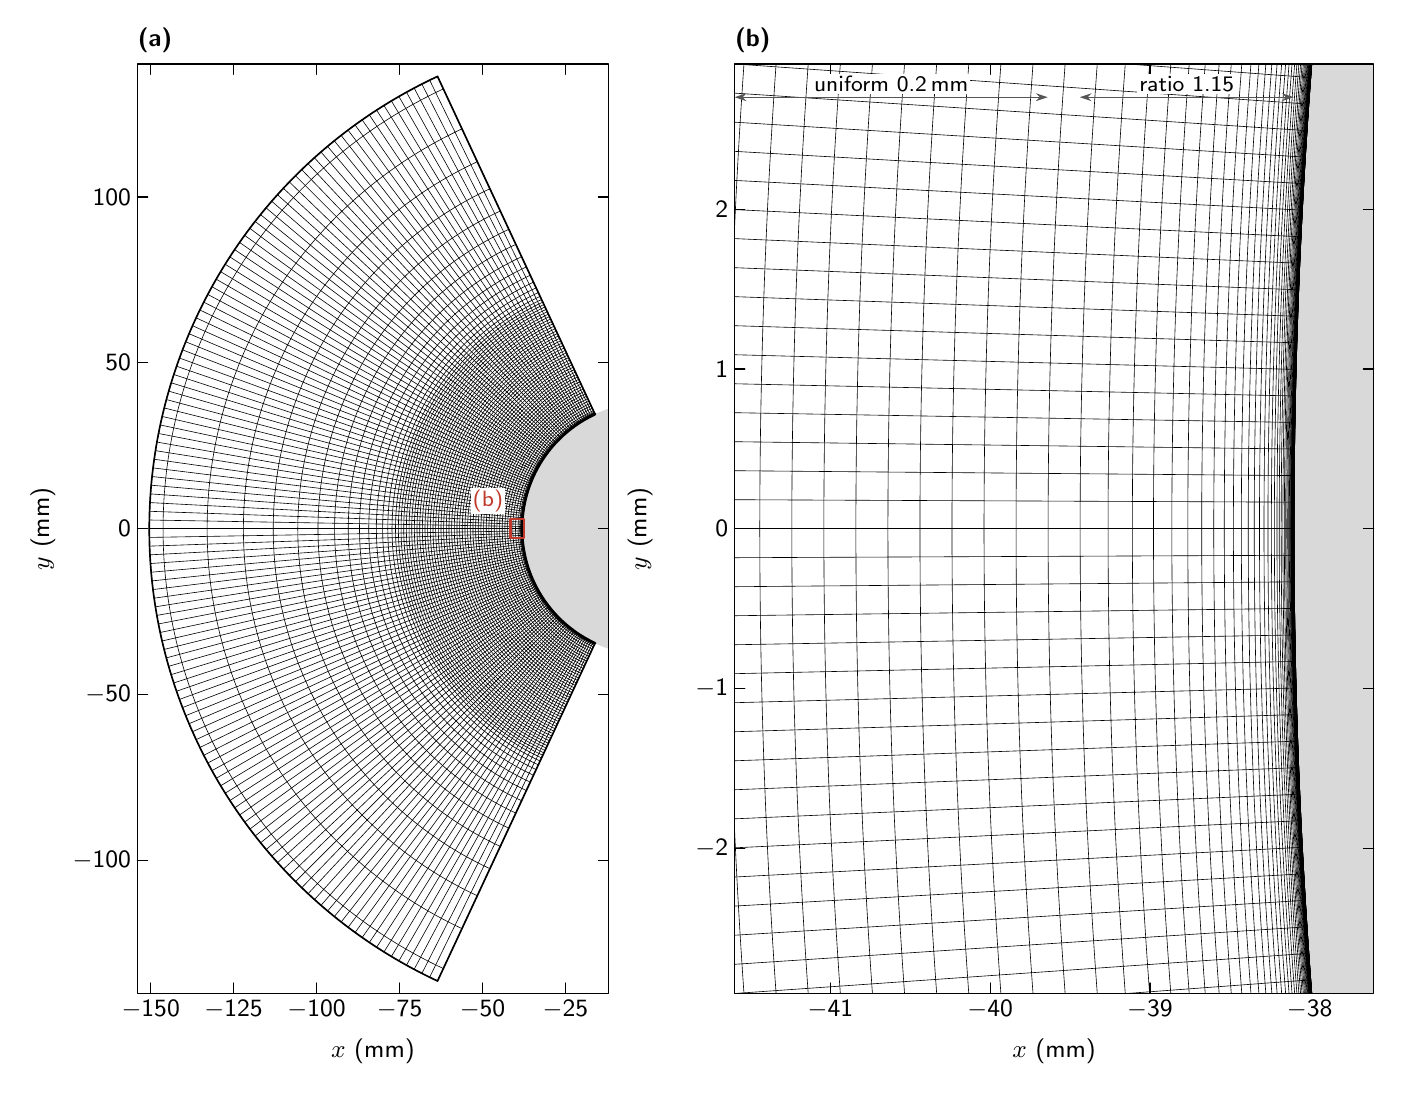
\begin{tikzpicture}[x=1mm, y=1mm, line cap=round, line join=round]
% (a) circles i = 0..294 step 4; rays j = 0..520 step 4
\begin{scope}[shift={(76.9,69)}, x=0.421429mm, y=0.421429mm]
  \begin{scope}
    \clip (-154,-140) rectangle (-12,140);
    \fill[bodygrey] (0,0) circle[radius=38.1];
    % circles r = r_i
    \draw[grid] (115:38.100609192) arc[start angle=115, end angle=245, radius=38.100609192];
    \draw[grid] (115:38.101674672) arc[start angle=115, end angle=245, radius=38.101674672];
    \draw[grid] (115:38.103538203) arc[start angle=115, end angle=245, radius=38.103538203];
    \draw[grid] (115:38.106797532) arc[start angle=115, end angle=245, radius=38.106797532];
    \draw[grid] (115:38.112498117) arc[start angle=115, end angle=245, radius=38.112498117];
    \draw[grid] (115:38.122468477) arc[start angle=115, end angle=245, radius=38.122468477];
    \draw[grid] (115:38.139906698) arc[start angle=115, end angle=245, radius=38.139906698];
    \draw[grid] (115:38.170406256) arc[start angle=115, end angle=245, radius=38.170406256];
    \draw[grid] (115:38.223750173) arc[start angle=115, end angle=245, radius=38.223750173];
    \draw[grid] (115:38.317049018) arc[start angle=115, end angle=245, radius=38.317049018];
    \draw[grid] (115:38.48022928) arc[start angle=115, end angle=245, radius=38.48022928];
    \draw[grid] (115:38.765632579) arc[start angle=115, end angle=245, radius=38.765632579];
    \draw[grid] (115:39.264804733) arc[start angle=115, end angle=245, radius=39.264804733];
    \draw[grid] (115:40.04122639) arc[start angle=115, end angle=245, radius=40.04122639];
    \draw[grid] (115:40.843331653) arc[start angle=115, end angle=245, radius=40.843331653];
    \draw[grid] (115:41.645436916) arc[start angle=115, end angle=245, radius=41.645436916];
    \draw[grid] (115:42.44754218) arc[start angle=115, end angle=245, radius=42.44754218];
    \draw[grid] (115:43.249647443) arc[start angle=115, end angle=245, radius=43.249647443];
    \draw[grid] (115:44.051752706) arc[start angle=115, end angle=245, radius=44.051752706];
    \draw[grid] (115:44.853857969) arc[start angle=115, end angle=245, radius=44.853857969];
    \draw[grid] (115:45.655963232) arc[start angle=115, end angle=245, radius=45.655963232];
    \draw[grid] (115:46.458068495) arc[start angle=115, end angle=245, radius=46.458068495];
    \draw[grid] (115:47.260173758) arc[start angle=115, end angle=245, radius=47.260173758];
    \draw[grid] (115:48.062279022) arc[start angle=115, end angle=245, radius=48.062279022];
    \draw[grid] (115:48.864384285) arc[start angle=115, end angle=245, radius=48.864384285];
    \draw[grid] (115:49.666489548) arc[start angle=115, end angle=245, radius=49.666489548];
    \draw[grid] (115:50.468594811) arc[start angle=115, end angle=245, radius=50.468594811];
    \draw[grid] (115:51.270700074) arc[start angle=115, end angle=245, radius=51.270700074];
    \draw[grid] (115:52.072805337) arc[start angle=115, end angle=245, radius=52.072805337];
    \draw[grid] (115:52.874910601) arc[start angle=115, end angle=245, radius=52.874910601];
    \draw[grid] (115:53.677015864) arc[start angle=115, end angle=245, radius=53.677015864];
    \draw[grid] (115:54.479121127) arc[start angle=115, end angle=245, radius=54.479121127];
    \draw[grid] (115:55.28122639) arc[start angle=115, end angle=245, radius=55.28122639];
    \draw[grid] (115:56.083331653) arc[start angle=115, end angle=245, radius=56.083331653];
    \draw[grid] (115:56.885436916) arc[start angle=115, end angle=245, radius=56.885436916];
    \draw[grid] (115:57.68754218) arc[start angle=115, end angle=245, radius=57.68754218];
    \draw[grid] (115:58.489647443) arc[start angle=115, end angle=245, radius=58.489647443];
    \draw[grid] (115:59.291752706) arc[start angle=115, end angle=245, radius=59.291752706];
    \draw[grid] (115:60.093857969) arc[start angle=115, end angle=245, radius=60.093857969];
    \draw[grid] (115:60.895963232) arc[start angle=115, end angle=245, radius=60.895963232];
    \draw[grid] (115:61.698068495) arc[start angle=115, end angle=245, radius=61.698068495];
    \draw[grid] (115:62.500173758) arc[start angle=115, end angle=245, radius=62.500173758];
    \draw[grid] (115:63.302279022) arc[start angle=115, end angle=245, radius=63.302279022];
    \draw[grid] (115:64.104384285) arc[start angle=115, end angle=245, radius=64.104384285];
    \draw[grid] (115:64.906489548) arc[start angle=115, end angle=245, radius=64.906489548];
    \draw[grid] (115:65.708594811) arc[start angle=115, end angle=245, radius=65.708594811];
    \draw[grid] (115:66.510700074) arc[start angle=115, end angle=245, radius=66.510700074];
    \draw[grid] (115:67.312805337) arc[start angle=115, end angle=245, radius=67.312805337];
    \draw[grid] (115:68.114910601) arc[start angle=115, end angle=245, radius=68.114910601];
    \draw[grid] (115:68.917015864) arc[start angle=115, end angle=245, radius=68.917015864];
    \draw[grid] (115:69.719121127) arc[start angle=115, end angle=245, radius=69.719121127];
    \draw[grid] (115:70.52122639) arc[start angle=115, end angle=245, radius=70.52122639];
    \draw[grid] (115:71.323331653) arc[start angle=115, end angle=245, radius=71.323331653];
    \draw[grid] (115:72.125436916) arc[start angle=115, end angle=245, radius=72.125436916];
    \draw[grid] (115:72.92754218) arc[start angle=115, end angle=245, radius=72.92754218];
    \draw[grid] (115:73.729647443) arc[start angle=115, end angle=245, radius=73.729647443];
    \draw[grid] (115:74.531752706) arc[start angle=115, end angle=245, radius=74.531752706];
    \draw[grid] (115:75.333857969) arc[start angle=115, end angle=245, radius=75.333857969];
    \draw[grid] (115:76.198151456) arc[start angle=115, end angle=245, radius=76.198151456];
    \draw[grid] (115:77.248705591) arc[start angle=115, end angle=245, radius=77.248705591];
    \draw[grid] (115:78.525660708) arc[start angle=115, end angle=245, radius=78.525660708];
    \draw[grid] (115:80.077807634) arc[start angle=115, end angle=245, radius=80.077807634];
    \draw[grid] (115:81.964451923) arc[start angle=115, end angle=245, radius=81.964451923];
    \draw[grid] (115:84.257679849) arc[start angle=115, end angle=245, radius=84.257679849];
    \draw[grid] (115:87.045112724) arc[start angle=115, end angle=245, radius=87.045112724];
    \draw[grid] (115:90.433254806) arc[start angle=115, end angle=245, radius=90.433254806];
    \draw[grid] (115:94.551562683) arc[start angle=115, end angle=245, radius=94.551562683];
    \draw[grid] (115:99.557391646) arc[start angle=115, end angle=245, radius=99.557391646];
    \draw[grid] (115:105.642008037) arc[start angle=115, end angle=245, radius=105.642008037];
    \draw[grid] (115:113.03789729) arc[start angle=115, end angle=245, radius=113.03789729];
    \draw[grid] (115:122.027646901) arc[start angle=115, end angle=245, radius=122.027646901];
    \draw[grid] (115:132.954743738) arc[start angle=115, end angle=245, radius=132.954743738];
    \draw[grid] (115:146.236698239) arc[start angle=115, end angle=245, radius=146.236698239];
    \draw[grid] (115:150.387226276) arc[start angle=115, end angle=245, radius=150.387226276];
    % rays phi = phi_j
    \draw[grid] (115:38.1) -- (115:150.3872);
    \draw[grid] (116:38.1) -- (116:150.3872);
    \draw[grid] (117:38.1) -- (117:150.3872);
    \draw[grid] (118:38.1) -- (118:150.3872);
    \draw[grid] (119:38.1) -- (119:150.3872);
    \draw[grid] (120:38.1) -- (120:150.3872);
    \draw[grid] (121:38.1) -- (121:150.3872);
    \draw[grid] (122:38.1) -- (122:150.3872);
    \draw[grid] (123:38.1) -- (123:150.3872);
    \draw[grid] (124:38.1) -- (124:150.3872);
    \draw[grid] (125:38.1) -- (125:150.3872);
    \draw[grid] (126:38.1) -- (126:150.3872);
    \draw[grid] (127:38.1) -- (127:150.3872);
    \draw[grid] (128:38.1) -- (128:150.3872);
    \draw[grid] (129:38.1) -- (129:150.3872);
    \draw[grid] (130:38.1) -- (130:150.3872);
    \draw[grid] (131:38.1) -- (131:150.3872);
    \draw[grid] (132:38.1) -- (132:150.3872);
    \draw[grid] (133:38.1) -- (133:150.3872);
    \draw[grid] (134:38.1) -- (134:150.3872);
    \draw[grid] (135:38.1) -- (135:150.3872);
    \draw[grid] (136:38.1) -- (136:150.3872);
    \draw[grid] (137:38.1) -- (137:150.3872);
    \draw[grid] (138:38.1) -- (138:150.3872);
    \draw[grid] (139:38.1) -- (139:150.3872);
    \draw[grid] (140:38.1) -- (140:150.3872);
    \draw[grid] (141:38.1) -- (141:150.3872);
    \draw[grid] (142:38.1) -- (142:150.3872);
    \draw[grid] (143:38.1) -- (143:150.3872);
    \draw[grid] (144:38.1) -- (144:150.3872);
    \draw[grid] (145:38.1) -- (145:150.3872);
    \draw[grid] (146:38.1) -- (146:150.3872);
    \draw[grid] (147:38.1) -- (147:150.3872);
    \draw[grid] (148:38.1) -- (148:150.3872);
    \draw[grid] (149:38.1) -- (149:150.3872);
    \draw[grid] (150:38.1) -- (150:150.3872);
    \draw[grid] (151:38.1) -- (151:150.3872);
    \draw[grid] (152:38.1) -- (152:150.3872);
    \draw[grid] (153:38.1) -- (153:150.3872);
    \draw[grid] (154:38.1) -- (154:150.3872);
    \draw[grid] (155:38.1) -- (155:150.3872);
    \draw[grid] (156:38.1) -- (156:150.3872);
    \draw[grid] (157:38.1) -- (157:150.3872);
    \draw[grid] (158:38.1) -- (158:150.3872);
    \draw[grid] (159:38.1) -- (159:150.3872);
    \draw[grid] (160:38.1) -- (160:150.3872);
    \draw[grid] (161:38.1) -- (161:150.3872);
    \draw[grid] (162:38.1) -- (162:150.3872);
    \draw[grid] (163:38.1) -- (163:150.3872);
    \draw[grid] (164:38.1) -- (164:150.3872);
    \draw[grid] (165:38.1) -- (165:150.3872);
    \draw[grid] (166:38.1) -- (166:150.3872);
    \draw[grid] (167:38.1) -- (167:150.3872);
    \draw[grid] (168:38.1) -- (168:150.3872);
    \draw[grid] (169:38.1) -- (169:150.3872);
    \draw[grid] (170:38.1) -- (170:150.3872);
    \draw[grid] (171:38.1) -- (171:150.3872);
    \draw[grid] (172:38.1) -- (172:150.3872);
    \draw[grid] (173:38.1) -- (173:150.3872);
    \draw[grid] (174:38.1) -- (174:150.3872);
    \draw[grid] (175:38.1) -- (175:150.3872);
    \draw[grid] (176:38.1) -- (176:150.3872);
    \draw[grid] (177:38.1) -- (177:150.3872);
    \draw[grid] (178:38.1) -- (178:150.3872);
    \draw[grid] (179:38.1) -- (179:150.3872);
    \draw[grid] (180:38.1) -- (180:150.3872);
    \draw[grid] (181:38.1) -- (181:150.3872);
    \draw[grid] (182:38.1) -- (182:150.3872);
    \draw[grid] (183:38.1) -- (183:150.3872);
    \draw[grid] (184:38.1) -- (184:150.3872);
    \draw[grid] (185:38.1) -- (185:150.3872);
    \draw[grid] (186:38.1) -- (186:150.3872);
    \draw[grid] (187:38.1) -- (187:150.3872);
    \draw[grid] (188:38.1) -- (188:150.3872);
    \draw[grid] (189:38.1) -- (189:150.3872);
    \draw[grid] (190:38.1) -- (190:150.3872);
    \draw[grid] (191:38.1) -- (191:150.3872);
    \draw[grid] (192:38.1) -- (192:150.3872);
    \draw[grid] (193:38.1) -- (193:150.3872);
    \draw[grid] (194:38.1) -- (194:150.3872);
    \draw[grid] (195:38.1) -- (195:150.3872);
    \draw[grid] (196:38.1) -- (196:150.3872);
    \draw[grid] (197:38.1) -- (197:150.3872);
    \draw[grid] (198:38.1) -- (198:150.3872);
    \draw[grid] (199:38.1) -- (199:150.3872);
    \draw[grid] (200:38.1) -- (200:150.3872);
    \draw[grid] (201:38.1) -- (201:150.3872);
    \draw[grid] (202:38.1) -- (202:150.3872);
    \draw[grid] (203:38.1) -- (203:150.3872);
    \draw[grid] (204:38.1) -- (204:150.3872);
    \draw[grid] (205:38.1) -- (205:150.3872);
    \draw[grid] (206:38.1) -- (206:150.3872);
    \draw[grid] (207:38.1) -- (207:150.3872);
    \draw[grid] (208:38.1) -- (208:150.3872);
    \draw[grid] (209:38.1) -- (209:150.3872);
    \draw[grid] (210:38.1) -- (210:150.3872);
    \draw[grid] (211:38.1) -- (211:150.3872);
    \draw[grid] (212:38.1) -- (212:150.3872);
    \draw[grid] (213:38.1) -- (213:150.3872);
    \draw[grid] (214:38.1) -- (214:150.3872);
    \draw[grid] (215:38.1) -- (215:150.3872);
    \draw[grid] (216:38.1) -- (216:150.3872);
    \draw[grid] (217:38.1) -- (217:150.3872);
    \draw[grid] (218:38.1) -- (218:150.3872);
    \draw[grid] (219:38.1) -- (219:150.3872);
    \draw[grid] (220:38.1) -- (220:150.3872);
    \draw[grid] (221:38.1) -- (221:150.3872);
    \draw[grid] (222:38.1) -- (222:150.3872);
    \draw[grid] (223:38.1) -- (223:150.3872);
    \draw[grid] (224:38.1) -- (224:150.3872);
    \draw[grid] (225:38.1) -- (225:150.3872);
    \draw[grid] (226:38.1) -- (226:150.3872);
    \draw[grid] (227:38.1) -- (227:150.3872);
    \draw[grid] (228:38.1) -- (228:150.3872);
    \draw[grid] (229:38.1) -- (229:150.3872);
    \draw[grid] (230:38.1) -- (230:150.3872);
    \draw[grid] (231:38.1) -- (231:150.3872);
    \draw[grid] (232:38.1) -- (232:150.3872);
    \draw[grid] (233:38.1) -- (233:150.3872);
    \draw[grid] (234:38.1) -- (234:150.3872);
    \draw[grid] (235:38.1) -- (235:150.3872);
    \draw[grid] (236:38.1) -- (236:150.3872);
    \draw[grid] (237:38.1) -- (237:150.3872);
    \draw[grid] (238:38.1) -- (238:150.3872);
    \draw[grid] (239:38.1) -- (239:150.3872);
    \draw[grid] (240:38.1) -- (240:150.3872);
    \draw[grid] (241:38.1) -- (241:150.3872);
    \draw[grid] (242:38.1) -- (242:150.3872);
    \draw[grid] (243:38.1) -- (243:150.3872);
    \draw[grid] (244:38.1) -- (244:150.3872);
    \draw[grid] (245:38.1) -- (245:150.3872);
    % boundaries: wall, inlet, outlets
    \draw[wall] (115:38.1) arc[start angle=115, end angle=245, radius=38.1];
    \draw[edge] (115:150.3872) arc[start angle=115, end angle=245, radius=150.3872];
    \draw[edge] (115:38.1) -- (115:150.3872);
    \draw[edge] (245:38.1) -- (245:150.3872);
    \draw[zoom] (-41.6,-2.9079) rectangle (-37.6,2.9079);
  \end{scope}
\end{scope}
\draw[frame] (12,10) rectangle (71.843,128);
\draw[tick] (13.686,10) -- ++(0,1.3) (13.686,128) -- ++(0,-1.3);
\node[ticklbl, anchor=north] at (13.686,9.6) {$-$150};
\draw[tick] (24.221,10) -- ++(0,1.3) (24.221,128) -- ++(0,-1.3);
\node[ticklbl, anchor=north] at (24.221,9.6) {$-$125};
\draw[tick] (34.757,10) -- ++(0,1.3) (34.757,128) -- ++(0,-1.3);
\node[ticklbl, anchor=north] at (34.757,9.6) {$-$100};
\draw[tick] (45.293,10) -- ++(0,1.3) (45.293,128) -- ++(0,-1.3);
\node[ticklbl, anchor=north] at (45.293,9.6) {$-$75};
\draw[tick] (55.829,10) -- ++(0,1.3) (55.829,128) -- ++(0,-1.3);
\node[ticklbl, anchor=north] at (55.829,9.6) {$-$50};
\draw[tick] (66.364,10) -- ++(0,1.3) (66.364,128) -- ++(0,-1.3);
\node[ticklbl, anchor=north] at (66.364,9.6) {$-$25};
\draw[tick] (12,26.857) -- ++(1.3,0) (71.843,26.857) -- ++(-1.3,0);
\node[ticklbl, anchor=east] at (11.6,26.857) {$-$100};
\draw[tick] (12,47.929) -- ++(1.3,0) (71.843,47.929) -- ++(-1.3,0);
\node[ticklbl, anchor=east] at (11.6,47.929) {$-$50};
\draw[tick] (12,69) -- ++(1.3,0) (71.843,69) -- ++(-1.3,0);
\node[ticklbl, anchor=east] at (11.6,69) {0};
\draw[tick] (12,90.071) -- ++(1.3,0) (71.843,90.071) -- ++(-1.3,0);
\node[ticklbl, anchor=east] at (11.6,90.071) {50};
\draw[tick] (12,111.143) -- ++(1.3,0) (71.843,111.143) -- ++(-1.3,0);
\node[ticklbl, anchor=east] at (11.6,111.143) {100};
\node[axlbl, anchor=north] at (41.921,4.6) {$x$ (mm)};
\node[axlbl, anchor=south, rotate=90] at (2,69) {$y$ (mm)};
\node[panel, anchor=south west] at (12,129.4) {(a)};
% (b) circles i = 0..65 step 1; rays j = 239..281 step 1
\begin{scope}[shift={(931.877,69)}, x=20.289286mm, y=20.289286mm]
  \begin{scope}
    \clip (-41.6,-2.9079) rectangle (-37.6,2.9079);
    \fill[bodygrey] (0,0) circle[radius=38.1];
    % circles r = r_i
    \draw[grid] (174.578:38.100122) arc[start angle=174.578, end angle=185.422, radius=38.100122];
    \draw[grid] (174.578:38.1002623) arc[start angle=174.578, end angle=185.422, radius=38.1002623];
    \draw[grid] (174.578:38.100423645) arc[start angle=174.578, end angle=185.422, radius=38.100423645];
    \draw[grid] (174.578:38.100609192) arc[start angle=174.578, end angle=185.422, radius=38.100609192];
    \draw[grid] (174.578:38.100822571) arc[start angle=174.578, end angle=185.422, radius=38.100822571];
    \draw[grid] (174.578:38.101067956) arc[start angle=174.578, end angle=185.422, radius=38.101067956];
    \draw[grid] (174.578:38.10135015) arc[start angle=174.578, end angle=185.422, radius=38.10135015];
    \draw[grid] (174.578:38.101674672) arc[start angle=174.578, end angle=185.422, radius=38.101674672];
    \draw[grid] (174.578:38.102047873) arc[start angle=174.578, end angle=185.422, radius=38.102047873];
    \draw[grid] (174.578:38.102477054) arc[start angle=174.578, end angle=185.422, radius=38.102477054];
    \draw[grid] (174.578:38.102970612) arc[start angle=174.578, end angle=185.422, radius=38.102970612];
    \draw[grid] (174.578:38.103538203) arc[start angle=174.578, end angle=185.422, radius=38.103538203];
    \draw[grid] (174.578:38.104190934) arc[start angle=174.578, end angle=185.422, radius=38.104190934];
    \draw[grid] (174.578:38.104941574) arc[start angle=174.578, end angle=185.422, radius=38.104941574];
    \draw[grid] (174.578:38.10580481) arc[start angle=174.578, end angle=185.422, radius=38.10580481];
    \draw[grid] (174.578:38.106797532) arc[start angle=174.578, end angle=185.422, radius=38.106797532];
    \draw[grid] (174.578:38.107939161) arc[start angle=174.578, end angle=185.422, radius=38.107939161];
    \draw[grid] (174.578:38.109252036) arc[start angle=174.578, end angle=185.422, radius=38.109252036];
    \draw[grid] (174.578:38.110761841) arc[start angle=174.578, end angle=185.422, radius=38.110761841];
    \draw[grid] (174.578:38.112498117) arc[start angle=174.578, end angle=185.422, radius=38.112498117];
    \draw[grid] (174.578:38.114494835) arc[start angle=174.578, end angle=185.422, radius=38.114494835];
    \draw[grid] (174.578:38.11679106) arc[start angle=174.578, end angle=185.422, radius=38.11679106];
    \draw[grid] (174.578:38.119431719) arc[start angle=174.578, end angle=185.422, radius=38.119431719];
    \draw[grid] (174.578:38.122468477) arc[start angle=174.578, end angle=185.422, radius=38.122468477];
    \draw[grid] (174.578:38.125960748) arc[start angle=174.578, end angle=185.422, radius=38.125960748];
    \draw[grid] (174.578:38.12997686) arc[start angle=174.578, end angle=185.422, radius=38.12997686];
    \draw[grid] (174.578:38.134595389) arc[start angle=174.578, end angle=185.422, radius=38.134595389];
    \draw[grid] (174.578:38.139906698) arc[start angle=174.578, end angle=185.422, radius=38.139906698];
    \draw[grid] (174.578:38.146014702) arc[start angle=174.578, end angle=185.422, radius=38.146014702];
    \draw[grid] (174.578:38.153038908) arc[start angle=174.578, end angle=185.422, radius=38.153038908];
    \draw[grid] (174.578:38.161116744) arc[start angle=174.578, end angle=185.422, radius=38.161116744];
    \draw[grid] (174.578:38.170406256) arc[start angle=174.578, end angle=185.422, radius=38.170406256];
    \draw[grid] (174.578:38.181089194) arc[start angle=174.578, end angle=185.422, radius=38.181089194];
    \draw[grid] (174.578:38.193374573) arc[start angle=174.578, end angle=185.422, radius=38.193374573];
    \draw[grid] (174.578:38.207502759) arc[start angle=174.578, end angle=185.422, radius=38.207502759];
    \draw[grid] (174.578:38.223750173) arc[start angle=174.578, end angle=185.422, radius=38.223750173];
    \draw[grid] (174.578:38.242434699) arc[start angle=174.578, end angle=185.422, radius=38.242434699];
    \draw[grid] (174.578:38.263921904) arc[start angle=174.578, end angle=185.422, radius=38.263921904];
    \draw[grid] (174.578:38.288632189) arc[start angle=174.578, end angle=185.422, radius=38.288632189];
    \draw[grid] (174.578:38.317049018) arc[start angle=174.578, end angle=185.422, radius=38.317049018];
    \draw[grid] (174.578:38.34972837) arc[start angle=174.578, end angle=185.422, radius=38.34972837];
    \draw[grid] (174.578:38.387309626) arc[start angle=174.578, end angle=185.422, radius=38.387309626];
    \draw[grid] (174.578:38.43052807) arc[start angle=174.578, end angle=185.422, radius=38.43052807];
    \draw[grid] (174.578:38.48022928) arc[start angle=174.578, end angle=185.422, radius=38.48022928];
    \draw[grid] (174.578:38.537385672) arc[start angle=174.578, end angle=185.422, radius=38.537385672];
    \draw[grid] (174.578:38.603115523) arc[start angle=174.578, end angle=185.422, radius=38.603115523];
    \draw[grid] (174.578:38.678704851) arc[start angle=174.578, end angle=185.422, radius=38.678704851];
    \draw[grid] (174.578:38.765632579) arc[start angle=174.578, end angle=185.422, radius=38.765632579];
    \draw[grid] (174.578:38.865599466) arc[start angle=174.578, end angle=185.422, radius=38.865599466];
    \draw[grid] (174.578:38.980561386) arc[start angle=174.578, end angle=185.422, radius=38.980561386];
    \draw[grid] (174.578:39.112767594) arc[start angle=174.578, end angle=185.422, radius=39.112767594];
    \draw[grid] (174.578:39.264804733) arc[start angle=174.578, end angle=185.422, radius=39.264804733];
    \draw[grid] (174.578:39.439647443) arc[start angle=174.578, end angle=185.422, radius=39.439647443];
    \draw[grid] (174.578:39.640173758) arc[start angle=174.578, end angle=185.422, radius=39.640173758];
    \draw[grid] (174.578:39.840700074) arc[start angle=174.578, end angle=185.422, radius=39.840700074];
    \draw[grid] (174.578:40.04122639) arc[start angle=174.578, end angle=185.422, radius=40.04122639];
    \draw[grid] (174.578:40.241752706) arc[start angle=174.578, end angle=185.422, radius=40.241752706];
    \draw[grid] (174.578:40.442279022) arc[start angle=174.578, end angle=185.422, radius=40.442279022];
    \draw[grid] (174.578:40.642805337) arc[start angle=174.578, end angle=185.422, radius=40.642805337];
    \draw[grid] (174.578:40.843331653) arc[start angle=174.578, end angle=185.422, radius=40.843331653];
    \draw[grid] (174.578:41.043857969) arc[start angle=174.578, end angle=185.422, radius=41.043857969];
    \draw[grid] (174.578:41.244384285) arc[start angle=174.578, end angle=185.422, radius=41.244384285];
    \draw[grid] (174.578:41.444910601) arc[start angle=174.578, end angle=185.422, radius=41.444910601];
    \draw[grid] (174.578:41.645436916) arc[start angle=174.578, end angle=185.422, radius=41.645436916];
    \draw[grid] (174.578:41.845963232) arc[start angle=174.578, end angle=185.422, radius=41.845963232];
    % rays phi = phi_j
    \draw[grid] (174.75:38.1) -- (174.75:41.846);
    \draw[grid] (175:38.1) -- (175:41.846);
    \draw[grid] (175.25:38.1) -- (175.25:41.846);
    \draw[grid] (175.5:38.1) -- (175.5:41.846);
    \draw[grid] (175.75:38.1) -- (175.75:41.846);
    \draw[grid] (176:38.1) -- (176:41.846);
    \draw[grid] (176.25:38.1) -- (176.25:41.846);
    \draw[grid] (176.5:38.1) -- (176.5:41.846);
    \draw[grid] (176.75:38.1) -- (176.75:41.846);
    \draw[grid] (177:38.1) -- (177:41.846);
    \draw[grid] (177.25:38.1) -- (177.25:41.846);
    \draw[grid] (177.5:38.1) -- (177.5:41.846);
    \draw[grid] (177.75:38.1) -- (177.75:41.846);
    \draw[grid] (178:38.1) -- (178:41.846);
    \draw[grid] (178.25:38.1) -- (178.25:41.846);
    \draw[grid] (178.5:38.1) -- (178.5:41.846);
    \draw[grid] (178.75:38.1) -- (178.75:41.846);
    \draw[grid] (179:38.1) -- (179:41.846);
    \draw[grid] (179.25:38.1) -- (179.25:41.846);
    \draw[grid] (179.5:38.1) -- (179.5:41.846);
    \draw[grid] (179.75:38.1) -- (179.75:41.846);
    \draw[grid] (180:38.1) -- (180:41.846);
    \draw[grid] (180.25:38.1) -- (180.25:41.846);
    \draw[grid] (180.5:38.1) -- (180.5:41.846);
    \draw[grid] (180.75:38.1) -- (180.75:41.846);
    \draw[grid] (181:38.1) -- (181:41.846);
    \draw[grid] (181.25:38.1) -- (181.25:41.846);
    \draw[grid] (181.5:38.1) -- (181.5:41.846);
    \draw[grid] (181.75:38.1) -- (181.75:41.846);
    \draw[grid] (182:38.1) -- (182:41.846);
    \draw[grid] (182.25:38.1) -- (182.25:41.846);
    \draw[grid] (182.5:38.1) -- (182.5:41.846);
    \draw[grid] (182.75:38.1) -- (182.75:41.846);
    \draw[grid] (183:38.1) -- (183:41.846);
    \draw[grid] (183.25:38.1) -- (183.25:41.846);
    \draw[grid] (183.5:38.1) -- (183.5:41.846);
    \draw[grid] (183.75:38.1) -- (183.75:41.846);
    \draw[grid] (184:38.1) -- (184:41.846);
    \draw[grid] (184.25:38.1) -- (184.25:41.846);
    \draw[grid] (184.5:38.1) -- (184.5:41.846);
    \draw[grid] (184.75:38.1) -- (184.75:41.846);
    \draw[grid] (185:38.1) -- (185:41.846);
    \draw[grid] (185.25:38.1) -- (185.25:41.846);
    % boundaries: wall, inlet, outlets
    \draw[wall] (115:38.1) arc[start angle=115, end angle=245, radius=38.1];
    \draw[edge] (115:150.3872) arc[start angle=115, end angle=245, radius=150.3872];
    \draw[edge] (115:38.1) -- (115:150.3872);
    \draw[edge] (245:38.1) -- (245:150.3872);
  \end{scope}
\end{scope}
\draw[frame] (87.843,10) rectangle (169,128);
\draw[tick] (100.016,10) -- ++(0,1.3) (100.016,128) -- ++(0,-1.3);
\node[ticklbl, anchor=north] at (100.016,9.6) {$-$41};
\draw[tick] (120.306,10) -- ++(0,1.3) (120.306,128) -- ++(0,-1.3);
\node[ticklbl, anchor=north] at (120.306,9.6) {$-$40};
\draw[tick] (140.595,10) -- ++(0,1.3) (140.595,128) -- ++(0,-1.3);
\node[ticklbl, anchor=north] at (140.595,9.6) {$-$39};
\draw[tick] (160.884,10) -- ++(0,1.3) (160.884,128) -- ++(0,-1.3);
\node[ticklbl, anchor=north] at (160.884,9.6) {$-$38};
\draw[tick] (87.843,28.421) -- ++(1.3,0) (169,28.421) -- ++(-1.3,0);
\node[ticklbl, anchor=east] at (87.443,28.421) {$-$2};
\draw[tick] (87.843,48.711) -- ++(1.3,0) (169,48.711) -- ++(-1.3,0);
\node[ticklbl, anchor=east] at (87.443,48.711) {$-$1};
\draw[tick] (87.843,69) -- ++(1.3,0) (169,69) -- ++(-1.3,0);
\node[ticklbl, anchor=east] at (87.443,69) {0};
\draw[tick] (87.843,89.289) -- ++(1.3,0) (169,89.289) -- ++(-1.3,0);
\node[ticklbl, anchor=east] at (87.443,89.289) {1};
\draw[tick] (87.843,109.579) -- ++(1.3,0) (169,109.579) -- ++(-1.3,0);
\node[ticklbl, anchor=east] at (87.443,109.579) {2};
\node[axlbl, anchor=north] at (128.421,4.6) {$x$ (mm)};
\node[axlbl, anchor=south, rotate=90] at (77.843,69) {$y$ (mm)};
\node[panel, anchor=south west] at (87.843,129.4) {(b)};
\node[note, text=accent, anchor=south east] at (58.769,70.825) {(b)};
\draw[dim] (127.606,123.8) -- (87.843,123.8);
\node[note, anchor=south] at (107.725,124.2) {uniform 0.2\,mm};
\draw[dim] (158.855,123.8) -- (131.675,123.8);
\node[note, anchor=south] at (145.265,124.2) {ratio 1.15};
\end{tikzpicture}
\end{document}
